\documentclass{article}

\usepackage{polski}
\usepackage[utf8]{inputenc}
\usepackage{booktabs}
\usepackage{biblatex}
\usepackage{subfigure}
\usepackage{graphicx}
\usepackage{float}
\usepackage{geometry}
\usepackage{listings}
\geometry{
	a4paper,
	total={170mm,257mm},
	left=50mm,
	right=50mm,
	top=45mm,
	bottom = 45mm
}
\usepackage{tabularx}


\begin{document}
	\newgeometry{tmargin=4cm, bmargin=4cm, lmargin=3cm, rmargin=3cm}
	
	\begin{titlepage}
		\center
		\newcommand{\HRule}{\rule{\linewidth}{0.6mm}}
		
		\textsc{\LARGE Politechnika Wrocławska}\\[1.5cm]
		\textsc{\Large Laboratorium}\\[0.5cm] 
		\textsc{\large Inteligencja Obliczeniowa i jej Zastosowania}\\[0.7cm] 

		\HRule \\[0.4cm]
		{ \huge \bfseries Algorytmy ewolucyjne i hybrydowe}\\[0.4cm]
		\HRule \\[1.5cm]
		
		\begin{minipage}{0.4\textwidth}
			\begin{flushleft} \large
				\emph{Authors:}\\
				Rafał \textsc{Pieniążek}\\
                Jakub \textsc{Pomykała}
			\end{flushleft}
		\end{minipage}
		~
		\begin{minipage}{0.4\textwidth}
			\begin{flushright} \large
				\emph{Supervisor:} \\
				prof. dr inż. Olgierd \textsc{Unold} 
			\end{flushright}
		\end{minipage}\\[4cm]

		{\large \today}\\[3cm]
		
		\vfill
		
	\end{titlepage}
\tableofcontents
\newpage
\listoffigures
\newpage
\section{Wstęp}
	Celem laboratorium było przeprowadzenie optymalizacji globalnej dla wybranych funkcji z pakietu globalOptTests.
    

\section{Zastosowany algorytm optymalizacji}

W laboratorium zastosowano algorytmy genetyczne będące klasa algorytmów ewolucyjnych.
Algorytmy ewolucyjne stanowią kierunek sztucznej inteligencji, która wykorzystuje i symuluje ewolucję biologiczną. Wszystkie algorytmy tej klasy symulują podstawowe zachowania w teorii ewolucji biologicznej - procesy selekcji, mutacji i reprodukcji. Zachowanie jednostek zależy od środowiska. Zbiór jednostek nazywa się populacją. Taka populacja ewoluuje zgodnie z regułami selekcji zgodnie z funkcją celu przypisaną do środowiska. Propagowane do kolejnych pokoleń są tylko najbardziej dopasowane osobniki.

\newpage
\section{Funkcja Aluffi - Pentini}
	\subsection{Wzór analityczny}
	   \begin{figure}[!htbp]
    \centering
    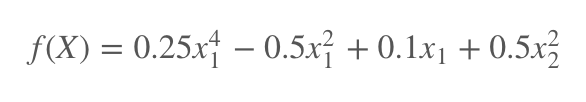
\includegraphics[width=0.7\textwidth]{inc/wzory/aluffi-pentini}
     \caption{Wzór analityczny funkcji Aluffi - Pentini}
    \end{figure}
    
    \subsection{Wykres w ustalonym przedziale zmiennych}
    
    \begin{figure}[!htbp]
    \centering
    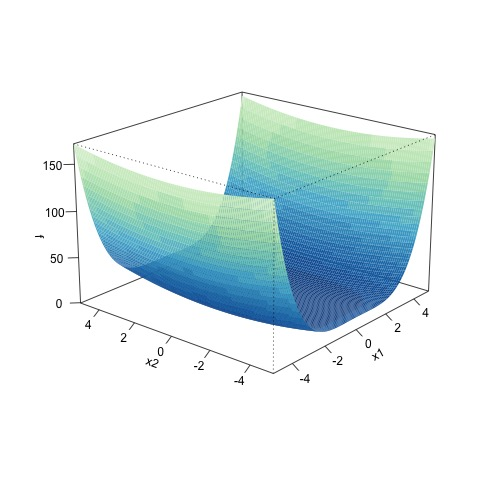
\includegraphics[width=0.7\textwidth]{inc/wykresyfunkcji/aluffi-pentini}
     \caption{Wykres  funkcji Aluffi - Pentini}
    \end{figure}
    
    
    \subsection{Optymalizacja poszukiwania ekstremum globalnego}

\subsubsection{Modyfikacja parametru elitarności}
\begin{figure}[!htbp]s
    \centering
\mbox{
\subfigure{
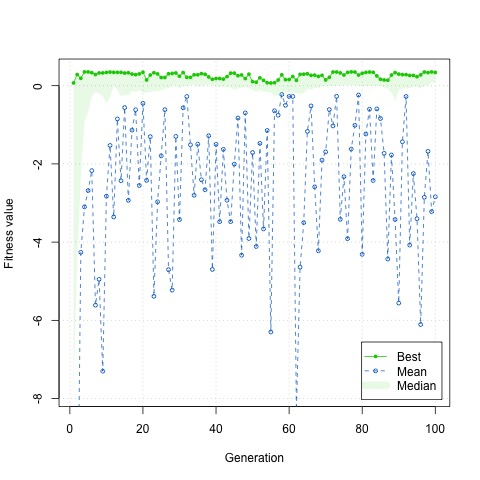
\includegraphics[width=3in]{{{inc/results/generations-AluffiPentini-p050-i100-c0.80-m0.10-e0.00}}}\quad
}
\subfigure{
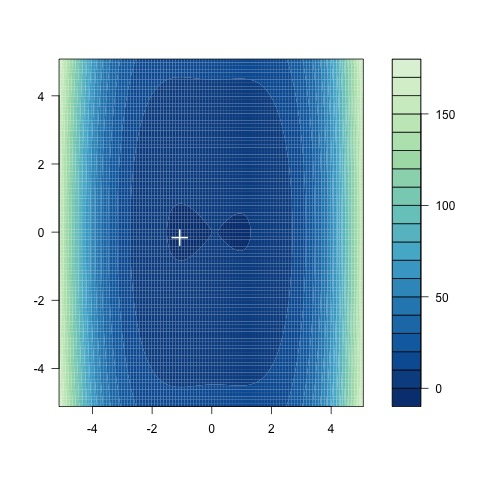
\includegraphics[width=3in]{{{inc/results/result-AluffiPentini-p050-i100-c0.80-m0.10-e0.00}}}\quad
}
}
                 \caption{Test optymalizacji GA AluffiPentini p50 i100 c0.8 m0.1 e0}
                 \end{figure}
\begin{figure}[!htbp]
    \centering
\mbox{
\subfigure{
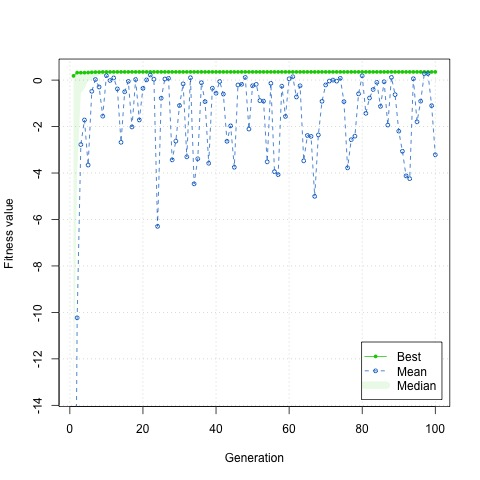
\includegraphics[width=3in]{{{inc/results/generations-AluffiPentini-p050-i100-c0.80-m0.10-e0.25}}}\quad
}
\subfigure{
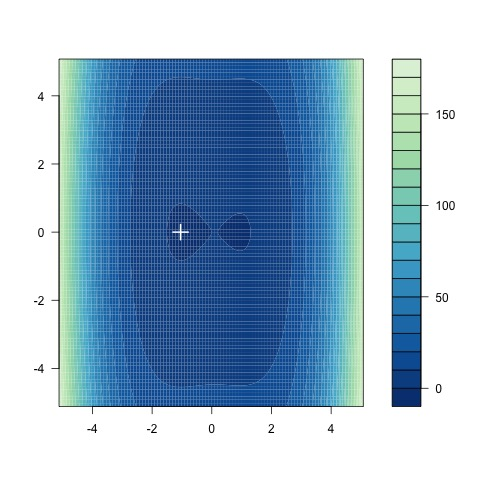
\includegraphics[width=3in]{{{inc/results/result-AluffiPentini-p050-i100-c0.80-m0.10-e0.25}}}\quad
}
}
                 \caption{Test optymalizacji GA AluffiPentini p50 i100 c0.8 m0.1 e0.25}
                 \end{figure}
\begin{figure}[!htbp]
    \centering
\mbox{
\subfigure{
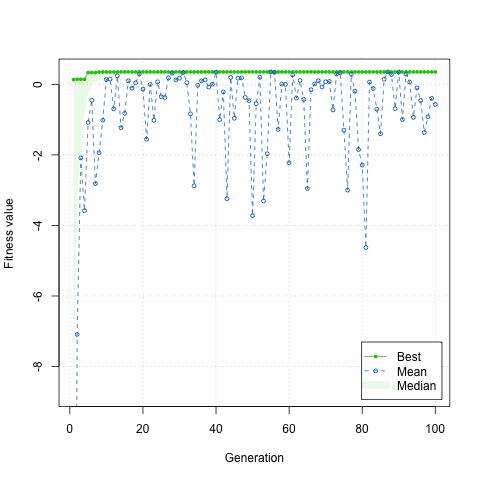
\includegraphics[width=3in]{{{inc/results/generations-AluffiPentini-p050-i100-c0.80-m0.10-e0.50}}}\quad
}
\subfigure{
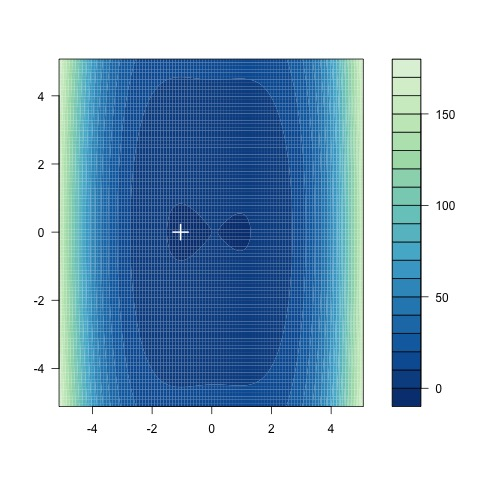
\includegraphics[width=3in]{{{inc/results/result-AluffiPentini-p050-i100-c0.80-m0.10-e0.50}}}\quad
}
}
                 \caption{Test optymalizacji GA AluffiPentini p50 i100 c0.8 m0.1 e0.5}
                 \end{figure}
\begin{figure}[!htbp]
    \centering
\mbox{
\subfigure{
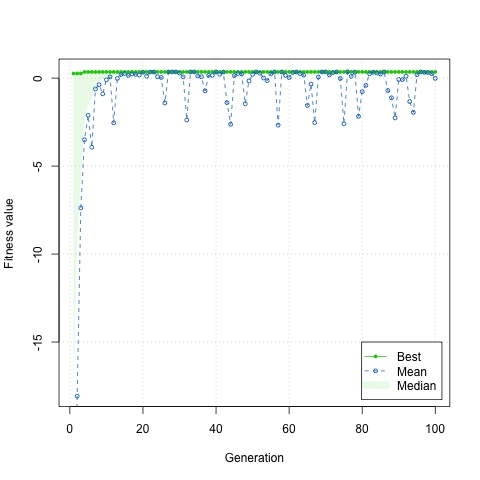
\includegraphics[width=3in]{{{inc/results/generations-AluffiPentini-p050-i100-c0.80-m0.10-e0.75}}}\quad
}
\subfigure{
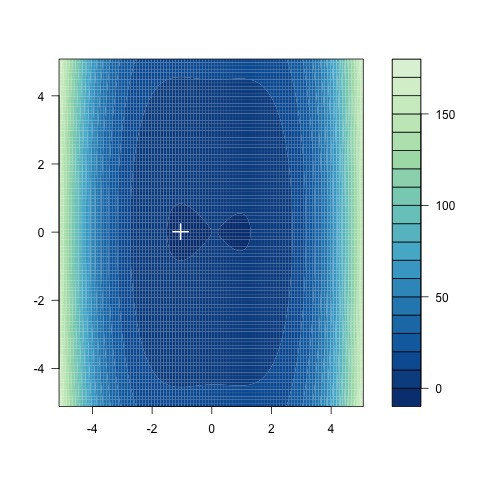
\includegraphics[width=3in]{{{inc/results/result-AluffiPentini-p050-i100-c0.80-m0.10-e0.75}}}\quad
}
}
                 \caption{Test optymalizacji GA AluffiPentini p50 i100 c0.8 m0.1 e0.75}
                 \end{figure}
\begin{figure}[!htbp]
    \centering
\mbox{
\subfigure{
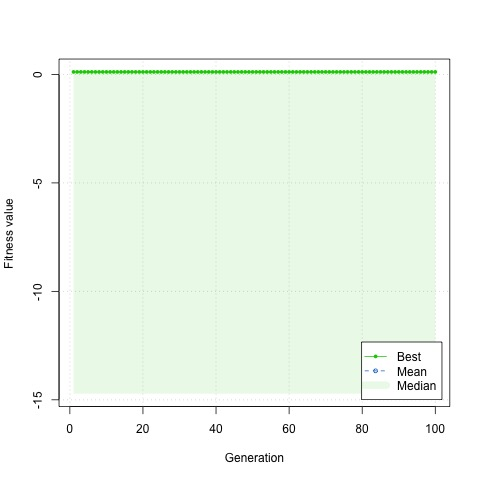
\includegraphics[width=3in]{{{inc/results/generations-AluffiPentini-p050-i100-c0.80-m0.10-e1.00}}}\quad
}
\subfigure{
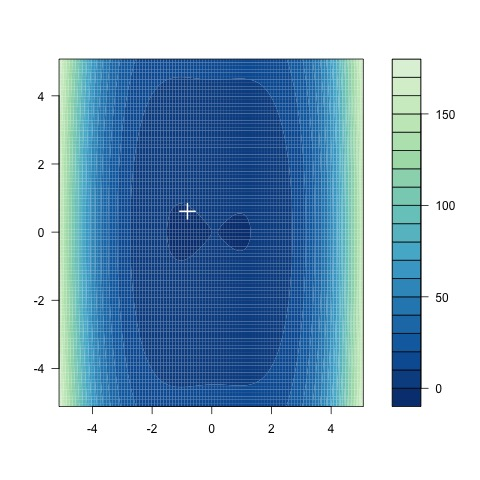
\includegraphics[width=3in]{{{inc/results/result-AluffiPentini-p050-i100-c0.80-m0.10-e1.00}}}\quad
}
}
                 \caption{Test optymalizacji GA AluffiPentini p50 i100 c0.8 m0.1 e1}
                 \end{figure}
\begin{figure}[!htbp]


\clearpage
\subsubsection{Modyfikacja parametru mutacji}
    \centering
\mbox{
\subfigure{
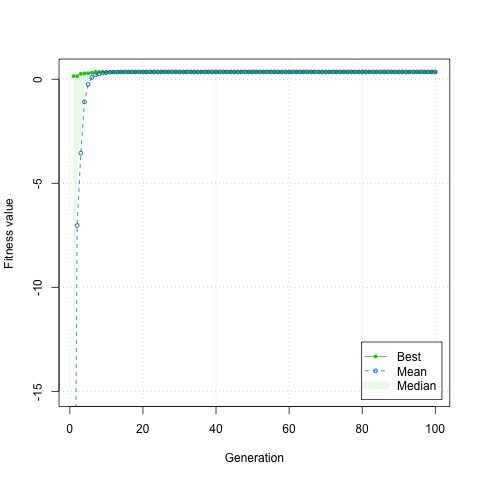
\includegraphics[width=3in]{{{inc/results/generations-AluffiPentini-p050-i100-c0.80-m0.00-e0.05}}}\quad
}
\subfigure{
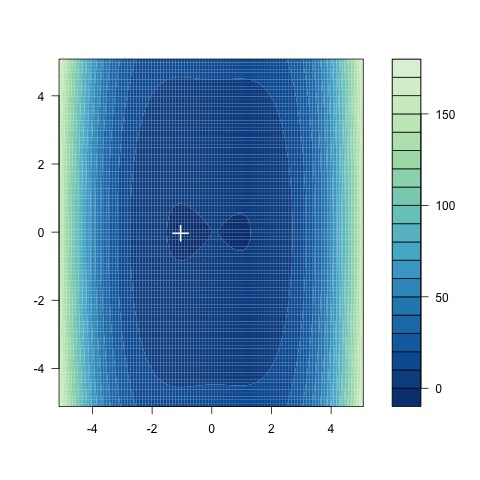
\includegraphics[width=3in]{{{inc/results/result-AluffiPentini-p050-i100-c0.80-m0.00-e0.05}}}\quad
}
}
                 \caption{Test optymalizacji GA AluffiPentini p50 i100 c0.8 m0 e0.05}
                 \end{figure}
\begin{figure}[!htbp]
    \centering
\mbox{
\subfigure{
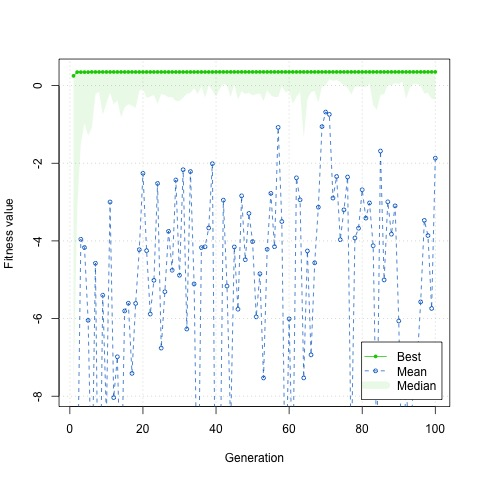
\includegraphics[width=3in]{{{inc/results/generations-AluffiPentini-p050-i100-c0.80-m0.25-e0.05}}}\quad
}
\subfigure{
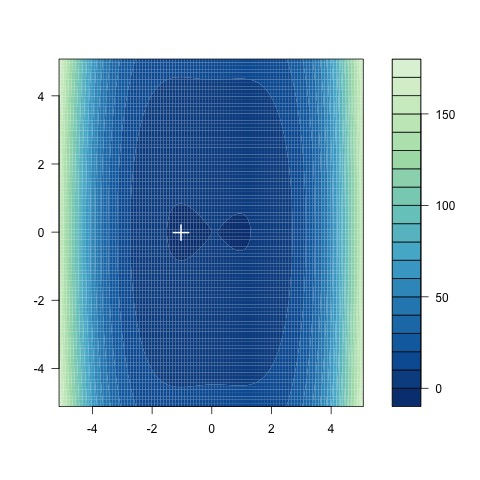
\includegraphics[width=3in]{{{inc/results/result-AluffiPentini-p050-i100-c0.80-m0.25-e0.05}}}\quad
}
}
                 \caption{Test optymalizacji GA AluffiPentini p50 i100 c0.8 m0.25 e0.05}
                 \end{figure}
\begin{figure}[!htbp]
    \centering
\mbox{
\subfigure{
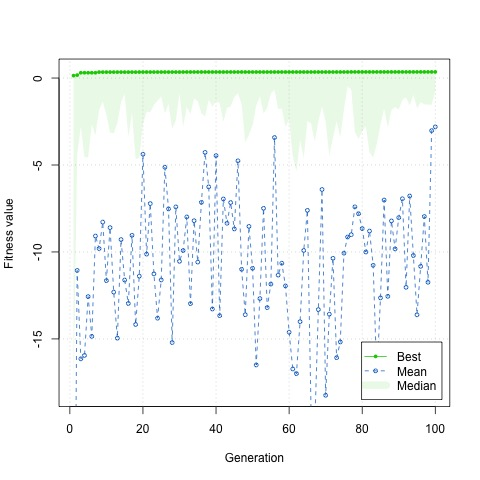
\includegraphics[width=3in]{{{inc/results/generations-AluffiPentini-p050-i100-c0.80-m0.50-e0.05}}}\quad
}
\subfigure{
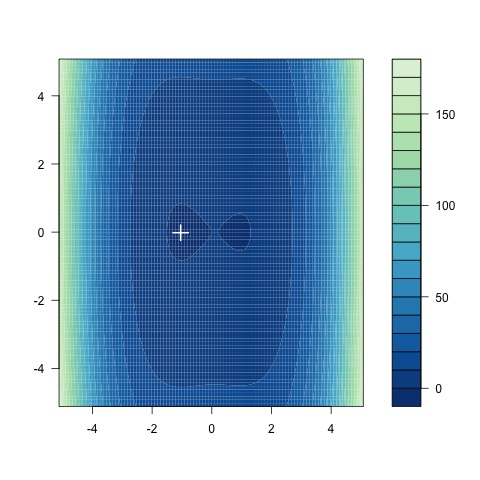
\includegraphics[width=3in]{{{inc/results/result-AluffiPentini-p050-i100-c0.80-m0.50-e0.05}}}\quad
}
}
                 \caption{Test optymalizacji GA AluffiPentini p50 i100 c0.8 m0.5 e0.05}
                 \end{figure}
\begin{figure}[!htbp]
    \centering
\mbox{
\subfigure{
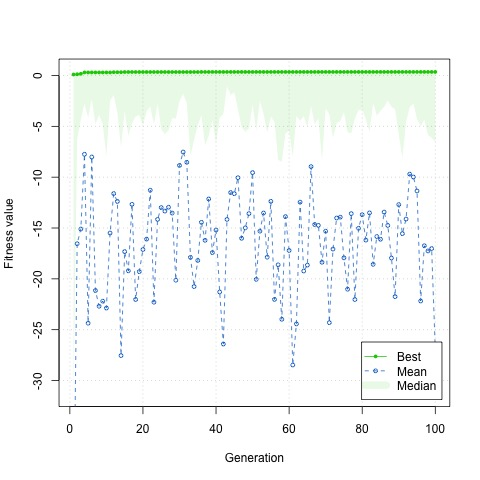
\includegraphics[width=3in]{{{inc/results/generations-AluffiPentini-p050-i100-c0.80-m0.75-e0.05}}}\quad
}
\subfigure{
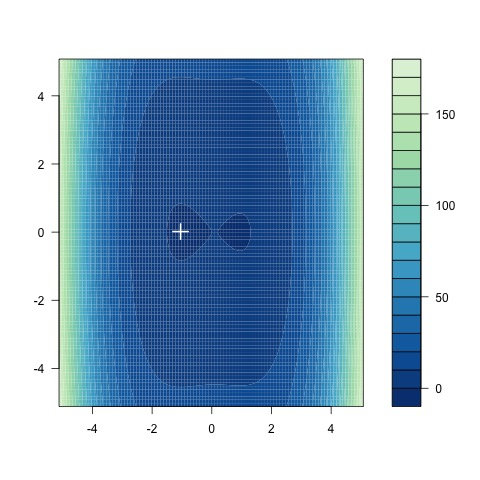
\includegraphics[width=3in]{{{inc/results/result-AluffiPentini-p050-i100-c0.80-m0.75-e0.05}}}\quad
}
}
                 \caption{Test optymalizacji GA AluffiPentini p50 i100 c0.8 m0.75 e0.05}
                 \end{figure}
\begin{figure}[!htbp]
    \centering
\mbox{
\subfigure{
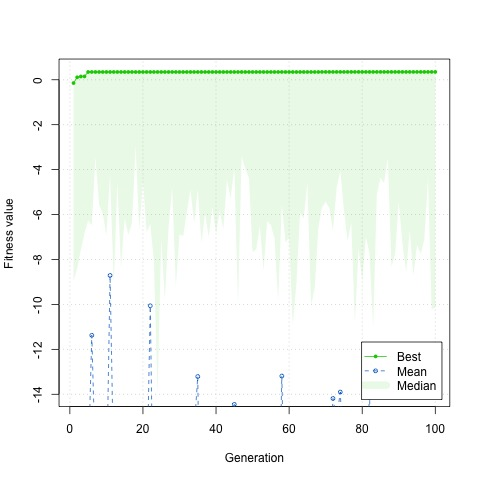
\includegraphics[width=3in]{{{inc/results/generations-AluffiPentini-p050-i100-c0.80-m1.00-e0.05}}}\quad
}
\subfigure{
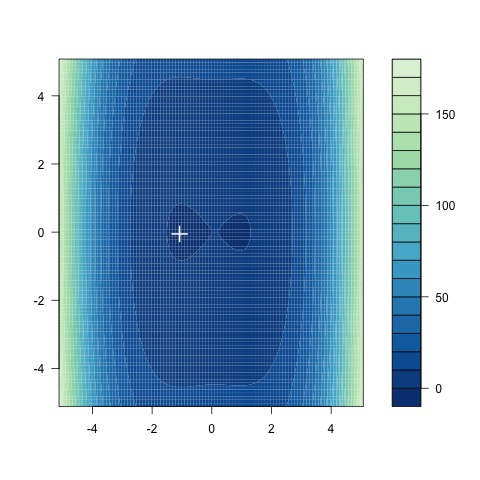
\includegraphics[width=3in]{{{inc/results/result-AluffiPentini-p050-i100-c0.80-m1.00-e0.05}}}\quad
}
}
                 \caption{Test optymalizacji GA AluffiPentini p50 i100 c0.8 m1 e0.05}
                 \end{figure}
                 
\clearpage
\subsubsection{Modyfikacja parametru krzyżowania}

\begin{figure}[!htbp]
    \centering
\mbox{
\subfigure{
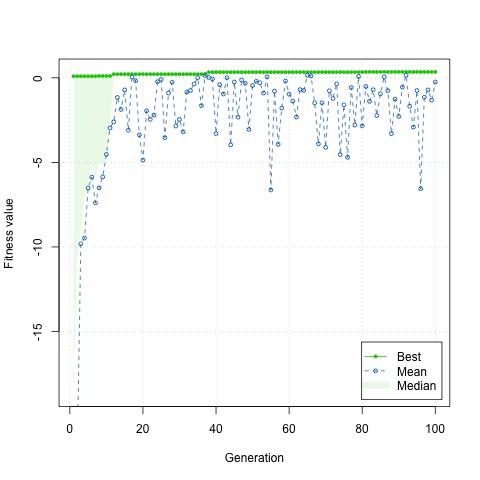
\includegraphics[width=3in]{{{inc/results/generations-AluffiPentini-p050-i100-c0.00-m0.10-e0.05}}}\quad
}
\subfigure{
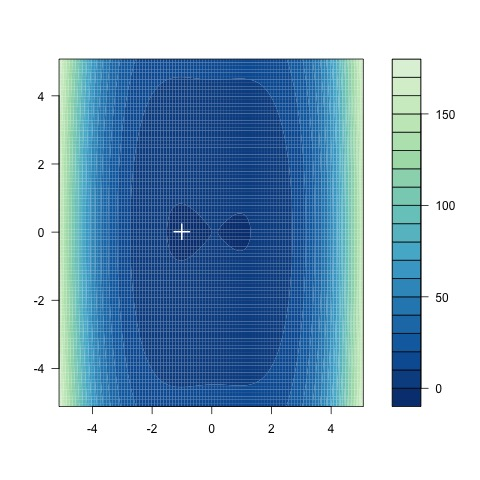
\includegraphics[width=3in]{{{inc/results/result-AluffiPentini-p050-i100-c0.00-m0.10-e0.05}}}\quad
}
}
                 \caption{Test optymalizacji GA AluffiPentini p50 i100 c0 m0.1 e0.05}
                 \end{figure}
\begin{figure}[!htbp]
    \centering
\mbox{
\subfigure{
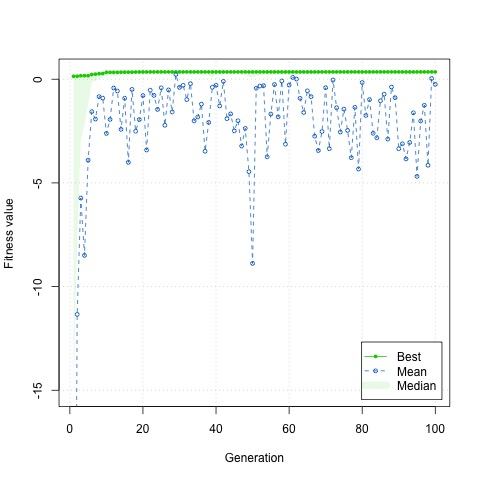
\includegraphics[width=3in]{{{inc/results/generations-AluffiPentini-p050-i100-c0.25-m0.10-e0.05}}}\quad
}
\subfigure{
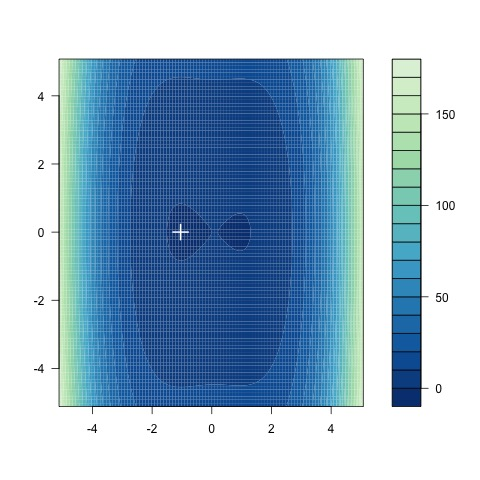
\includegraphics[width=3in]{{{inc/results/result-AluffiPentini-p050-i100-c0.25-m0.10-e0.05}}}\quad
}
}
                 \caption{Test optymalizacji GA AluffiPentini p50 i100 c0.25 m0.1 e0.05}
                 \end{figure}
\begin{figure}[!htbp]
    \centering
\mbox{
\subfigure{
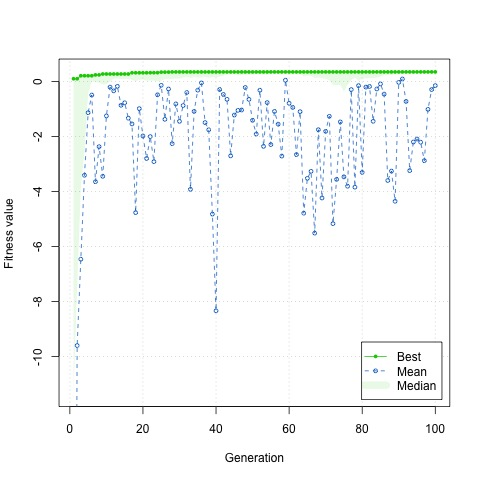
\includegraphics[width=3in]{{{inc/results/generations-AluffiPentini-p050-i100-c0.50-m0.10-e0.05}}}\quad
}
\subfigure{
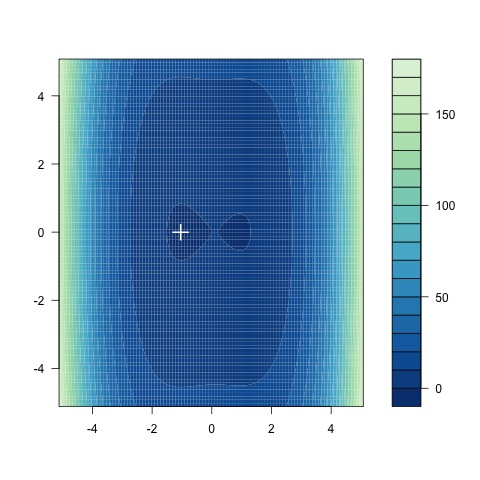
\includegraphics[width=3in]{{{inc/results/result-AluffiPentini-p050-i100-c0.50-m0.10-e0.05}}}\quad
}
}
                 \caption{Test optymalizacji GA AluffiPentini p50 i100 c0.5 m0.1 e0.05}
                 \end{figure}
\begin{figure}[!htbp]
    \centering
\mbox{
\subfigure{
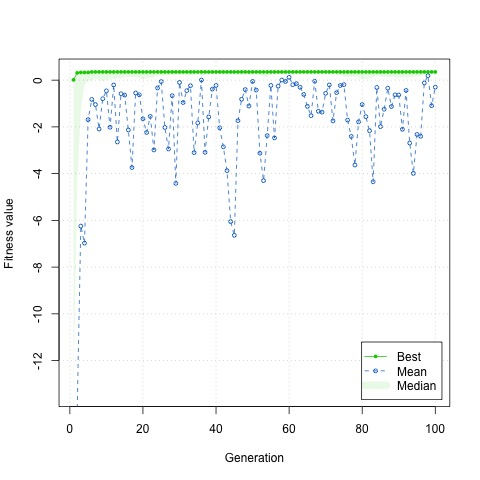
\includegraphics[width=3in]{{{inc/results/generations-AluffiPentini-p050-i100-c0.75-m0.10-e0.05}}}\quad
}
\subfigure{
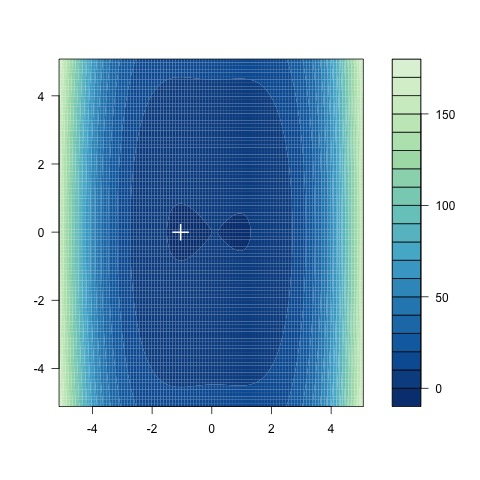
\includegraphics[width=3in]{{{inc/results/result-AluffiPentini-p050-i100-c0.75-m0.10-e0.05}}}\quad
}
}
                 \caption{Test optymalizacji GA AluffiPentini p50 i100 c0.75 m0.1 e0.05}
                 \end{figure}
\begin{figure}[!htbp]
    \centering
\mbox{
\subfigure{
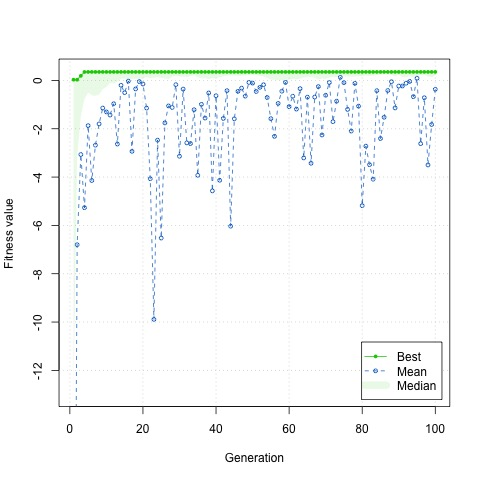
\includegraphics[width=3in]{{{inc/results/generations-AluffiPentini-p050-i100-c1.00-m0.10-e0.05}}}\quad
}
\subfigure{
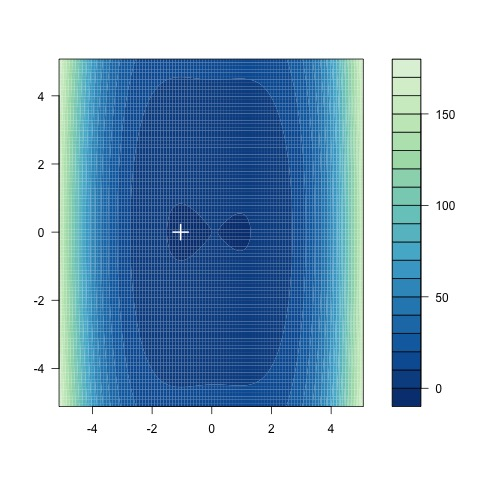
\includegraphics[width=3in]{{{inc/results/result-AluffiPentini-p050-i100-c1.00-m0.10-e0.05}}}\quad
}
}
                 \caption{Test optymalizacji GA AluffiPentini p50 i100 c1 m0.1 e0.05}
                 \end{figure}
                 
  \clearpage
\subsubsection{Modyfikacja parametru liczby iteracji}                    
\begin{figure}[!htbp]
    \centering
\mbox{
\subfigure{
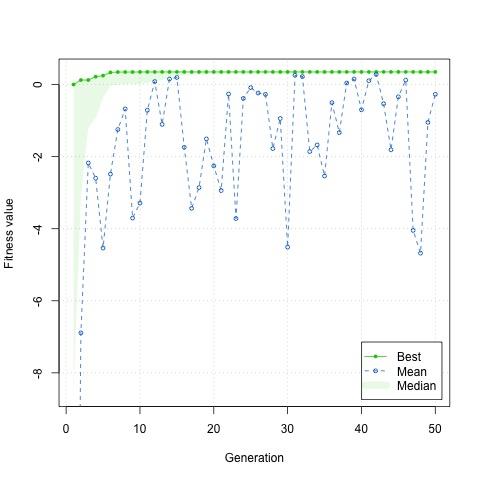
\includegraphics[width=3in]{{{inc/results/generations-AluffiPentini-p050-i050-c0.80-m0.10-e0.05}}}\quad
}
\subfigure{
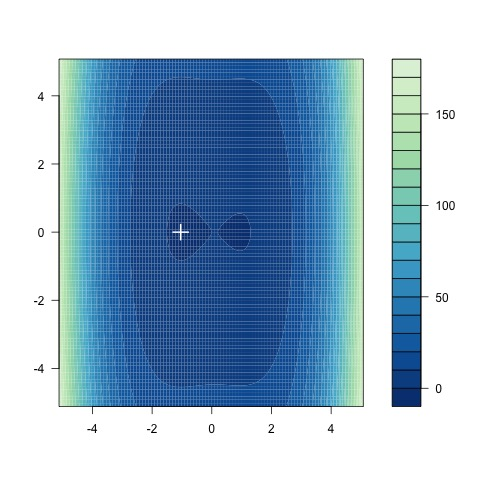
\includegraphics[width=3in]{{{inc/results/result-AluffiPentini-p050-i050-c0.80-m0.10-e0.05}}}\quad
}
}
                 \caption{Test optymalizacji GA AluffiPentini p50 i50 c0.8 m0.1 e0.05}
                 \end{figure}
\begin{figure}[!htbp]
    \centering
\mbox{
\subfigure{
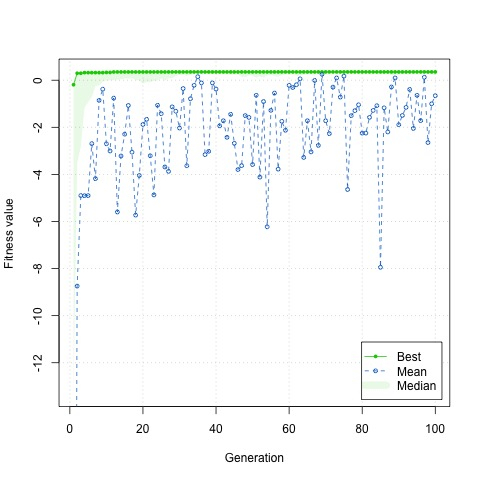
\includegraphics[width=3in]{{{inc/results/generations-AluffiPentini-p050-i100-c0.80-m0.10-e0.05}}}\quad
}
\subfigure{
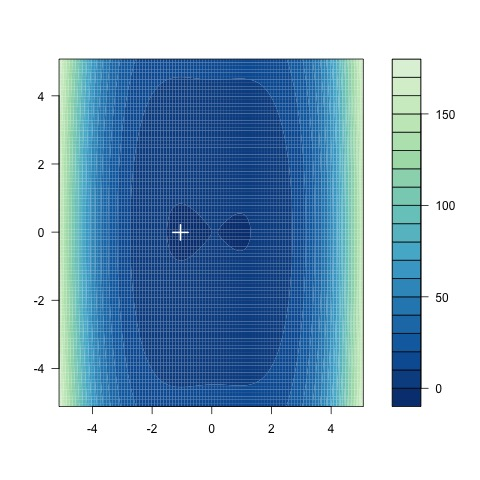
\includegraphics[width=3in]{{{inc/results/result-AluffiPentini-p050-i100-c0.80-m0.10-e0.05}}}\quad
}
}
                 \caption{Test optymalizacji GA AluffiPentini p50 i100 c0.8 m0.1 e0.05}
                 \end{figure}
\begin{figure}[!htbp]
    \centering
\mbox{
\subfigure{
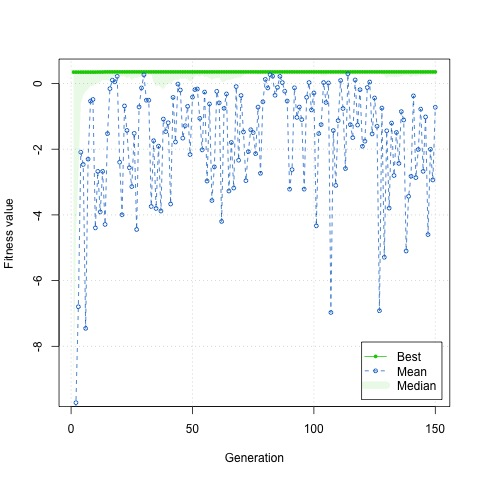
\includegraphics[width=3in]{{{inc/results/generations-AluffiPentini-p050-i150-c0.80-m0.10-e0.05}}}\quad
}
\subfigure{
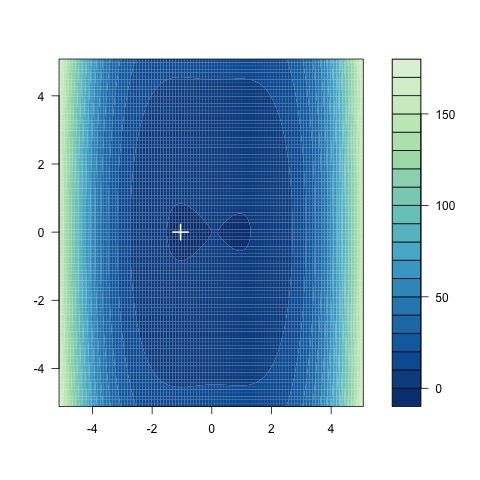
\includegraphics[width=3in]{{{inc/results/result-AluffiPentini-p050-i150-c0.80-m0.10-e0.05}}}\quad
}
}
                 \caption{Test optymalizacji GA AluffiPentini p50 i150 c0.8 m0.1 e0.05}
                 \end{figure}
\begin{figure}[!htbp]
    \centering
\mbox{
\subfigure{
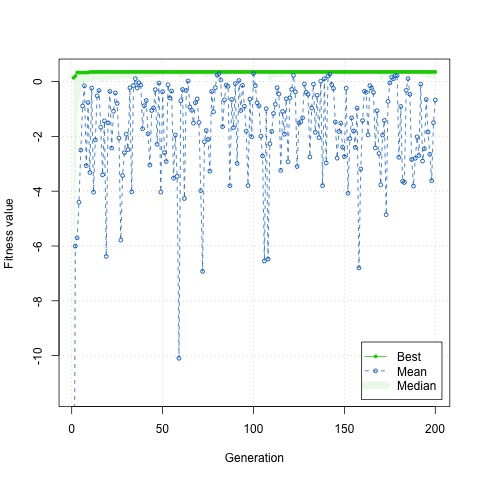
\includegraphics[width=3in]{{{inc/results/generations-AluffiPentini-p050-i200-c0.80-m0.10-e0.05}}}\quad
}
\subfigure{
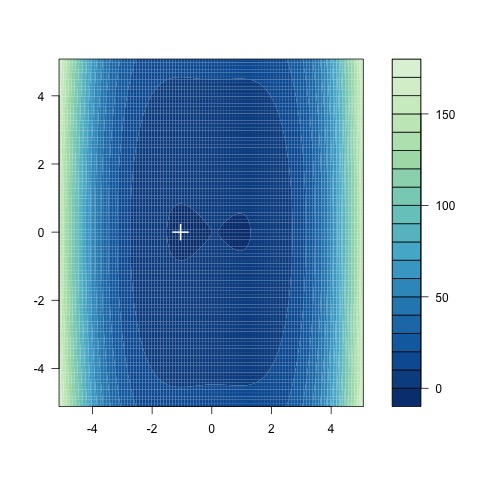
\includegraphics[width=3in]{{{inc/results/result-AluffiPentini-p050-i200-c0.80-m0.10-e0.05}}}\quad
}
}
                 \caption{Test optymalizacji GA AluffiPentini p50 i200 c0.8 m0.1 e0.05}
                 \end{figure}
\begin{figure}[!htbp]
    \centering
\mbox{
\subfigure{
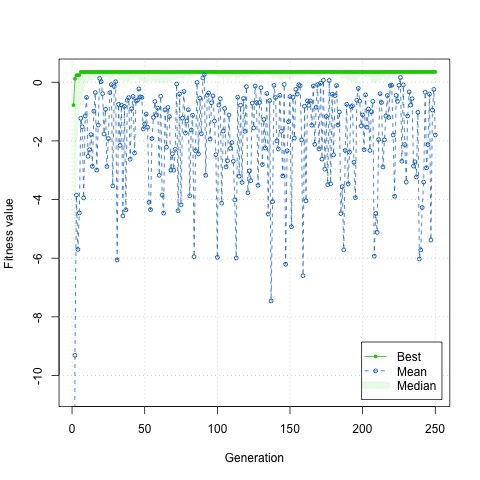
\includegraphics[width=3in]{{{inc/results/generations-AluffiPentini-p050-i250-c0.80-m0.10-e0.05}}}\quad
}
\subfigure{
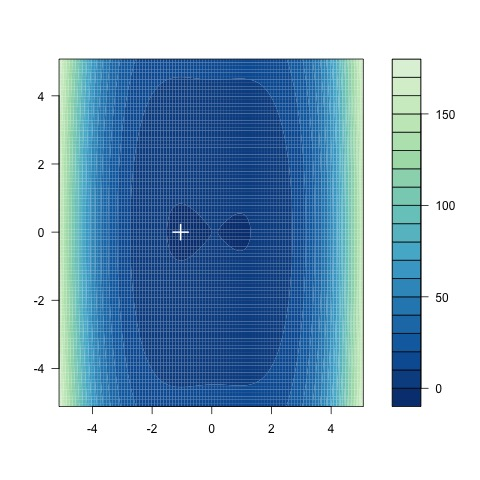
\includegraphics[width=3in]{{{inc/results/result-AluffiPentini-p050-i250-c0.80-m0.10-e0.05}}}\quad
}
}
                 \caption{Test optymalizacji GA AluffiPentini p50 i250 c0.8 m0.1 e0.05}
                 \end{figure}
                 
\clearpage
\subsubsection{Modyfikacja parametru rozmiaru populacji}              

\begin{figure}[!htbp]
    \centering
\mbox{
\subfigure{
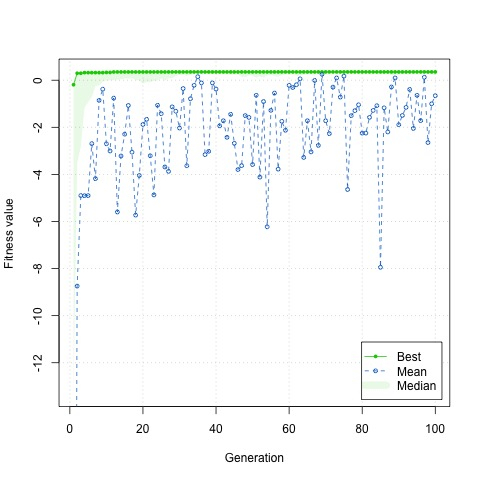
\includegraphics[width=3in]{{{inc/results/generations-AluffiPentini-p050-i100-c0.80-m0.10-e0.05}}}\quad
}
\subfigure{
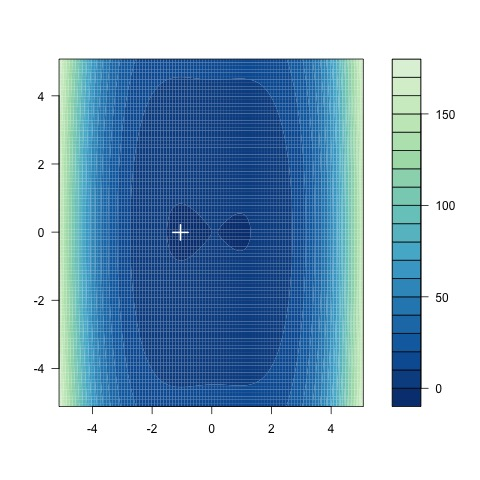
\includegraphics[width=3in]{{{inc/results/result-AluffiPentini-p050-i100-c0.80-m0.10-e0.05}}}\quad
}
}
                 \caption{Test optymalizacji GA AluffiPentini p50 i100 c0.8 m0.1 e0.05}
                 \end{figure}
\begin{figure}[!htbp]
    \centering
\mbox{
\subfigure{
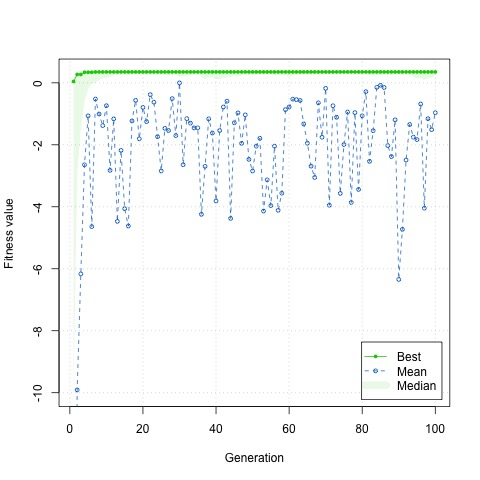
\includegraphics[width=3in]{{{inc/results/generations-AluffiPentini-p100-i100-c0.80-m0.10-e0.05}}}\quad
}
\subfigure{
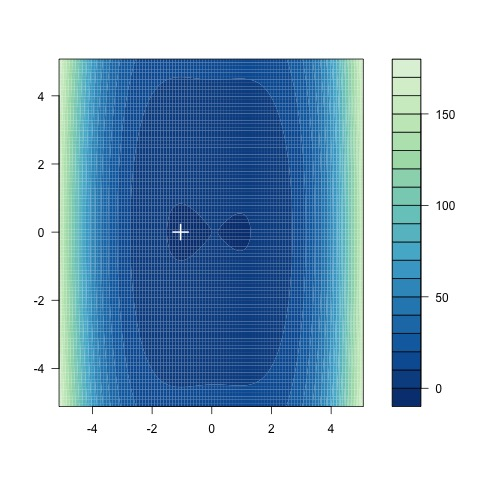
\includegraphics[width=3in]{{{inc/results/result-AluffiPentini-p100-i100-c0.80-m0.10-e0.05}}}\quad
}
}
                 \caption{Test optymalizacji GA AluffiPentini p100 i100 c0.8 m0.1 e0.05}
                 \end{figure}
\begin{figure}[!htbp]
    \centering
\mbox{
\subfigure{
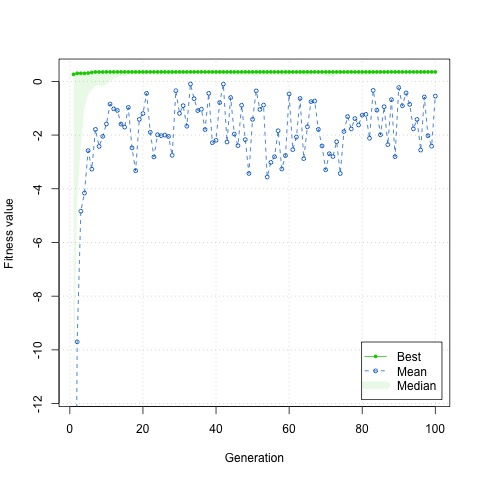
\includegraphics[width=3in]{{{inc/results/generations-AluffiPentini-p150-i100-c0.80-m0.10-e0.05}}}\quad
}
\subfigure{
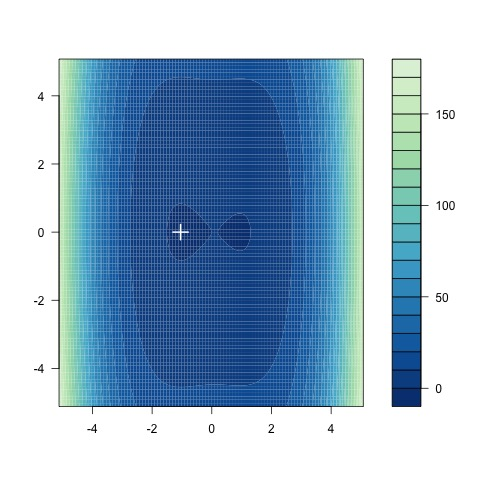
\includegraphics[width=3in]{{{inc/results/result-AluffiPentini-p150-i100-c0.80-m0.10-e0.05}}}\quad
}
}
                 \caption{Test optymalizacji GA AluffiPentini p150 i100 c0.8 m0.1 e0.05}
                 \end{figure}
\begin{figure}[!htbp]
    \centering
\mbox{
\subfigure{
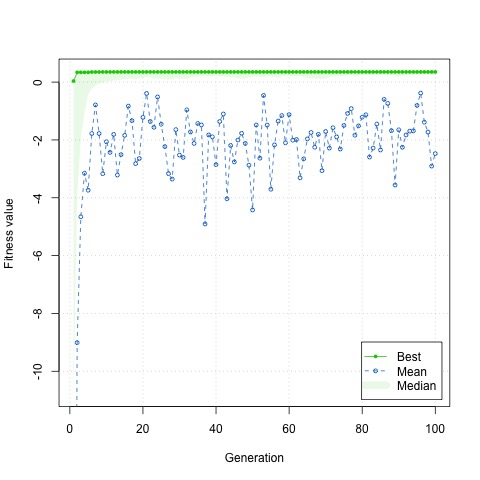
\includegraphics[width=3in]{{{inc/results/generations-AluffiPentini-p200-i100-c0.80-m0.10-e0.05}}}\quad
}
\subfigure{
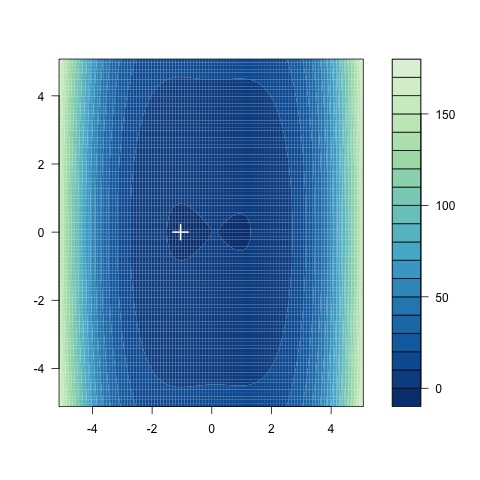
\includegraphics[width=3in]{{{inc/results/result-AluffiPentini-p200-i100-c0.80-m0.10-e0.05}}}\quad
}
}
                 \caption{Test optymalizacji GA AluffiPentini p200 i100 c0.8 m0.1 e0.05}
                 \end{figure}
                     \clearpage
\begin{figure}[!htbp]
    \centering
\mbox{
\subfigure{
\includegraphics[width=3in]{{{inc/results/generations-AluffiPentini-p250-i100-c0.80-m0.10-e0.05}}}\quad
}
\subfigure{
\includegraphics[width=3in]{{{inc/results/result-AluffiPentini-p250-i100-c0.80-m0.10-e0.05}}}\quad
}
}
                 \caption{Test optymalizacji GA AluffiPentini p250 i100 c0.8 m0.1 e0.05}
                 \end{figure}
                 
                 
                 
                 
                 
                 
\newpage
\section{Funkcja Bohachevsky'ego}
\subsection{Wzór analityczny}
\begin{figure}[!htbp]
    \centering
    \includegraphics[width=0.7\textwidth]{inc/wzory/bohachevsky}
     \caption{Wzór analityczny funkcji Bochachevsky'ego}
    \end{figure}
    
    \subsection{Wykres funkcji}
    \begin{figure}[!htbp]
    \centering
    \includegraphics[width=0.7\textwidth]{inc/wykresyfunkcji/bohachevsky}
     \caption{Wzór analityczny funkcji Bochachevsky'ego}
    \end{figure}
    
    \subsection{Optymalizacja}
\subsubsection{Modyfikacja parametru elitarności}    
\begin{figure}[!htbp]
    \centering
\mbox{
\subfigure{
\includegraphics[width=3in]{{{inc/results/generations-Bohachevsky1-p050-i100-c0.80-m0.10-e0.00}}}\quad
}
\subfigure{
\includegraphics[width=3in]{{{inc/results/result-Bohachevsky1-p050-i100-c0.80-m0.10-e0.00}}}\quad
}
}
                 \caption{Test optymalizacji GA Bohachevsky1 p50 i100 c0.8 m0.1 e0}
                 \end{figure}
\begin{figure}[!htbp]
    \centering
\mbox{
\subfigure{
\includegraphics[width=3in]{{{inc/results/generations-Bohachevsky1-p050-i100-c0.80-m0.10-e0.25}}}\quad
}
\subfigure{
\includegraphics[width=3in]{{{inc/results/result-Bohachevsky1-p050-i100-c0.80-m0.10-e0.25}}}\quad
}
}
                 \caption{Test optymalizacji GA Bohachevsky1 p50 i100 c0.8 m0.1 e0.25}
                 \end{figure}
\begin{figure}[!htbp]
    \centering
\mbox{
\subfigure{
\includegraphics[width=3in]{{{inc/results/generations-Bohachevsky1-p050-i100-c0.80-m0.10-e0.50}}}\quad
}
\subfigure{
\includegraphics[width=3in]{{{inc/results/result-Bohachevsky1-p050-i100-c0.80-m0.10-e0.50}}}\quad
}
}
                 \caption{Test optymalizacji GA Bohachevsky1 p50 i100 c0.8 m0.1 e0.5}
                 \end{figure}
\begin{figure}[!htbp]
    \centering
\mbox{
\subfigure{
\includegraphics[width=3in]{{{inc/results/generations-Bohachevsky1-p050-i100-c0.80-m0.10-e0.75}}}\quad
}
\subfigure{
\includegraphics[width=3in]{{{inc/results/result-Bohachevsky1-p050-i100-c0.80-m0.10-e0.75}}}\quad
}
}
                 \caption{Test optymalizacji GA Bohachevsky1 p50 i100 c0.8 m0.1 e0.75}
                 \end{figure}
\begin{figure}[!htbp]
    \centering
\mbox{
\subfigure{
\includegraphics[width=3in]{{{inc/results/generations-Bohachevsky1-p050-i100-c0.80-m0.10-e1.00}}}\quad
}
\subfigure{
\includegraphics[width=3in]{{{inc/results/result-Bohachevsky1-p050-i100-c0.80-m0.10-e1.00}}}\quad
}
}
                 \caption{Test optymalizacji GA Bohachevsky1 p50 i100 c0.8 m0.1 e1}
                 \end{figure}
                 
\clearpage
\subsubsection{Modyfikacja parametru mutacji}
\begin{figure}[!htbp]
    \centering
\mbox{
\subfigure{
\includegraphics[width=3in]{{{inc/results/generations-Bohachevsky1-p050-i100-c0.80-m0.00-e0.05}}}\quad
}
\subfigure{
\includegraphics[width=3in]{{{inc/results/result-Bohachevsky1-p050-i100-c0.80-m0.00-e0.05}}}\quad
}
}
                 \caption{Test optymalizacji GA Bohachevsky1 p50 i100 c0.8 m0 e0.05}
                 \end{figure}
\begin{figure}[!htbp]
    \centering
\mbox{
\subfigure{
\includegraphics[width=3in]{{{inc/results/generations-Bohachevsky1-p050-i100-c0.80-m0.25-e0.05}}}\quad
}
\subfigure{
\includegraphics[width=3in]{{{inc/results/result-Bohachevsky1-p050-i100-c0.80-m0.25-e0.05}}}\quad
}
}
                 \caption{Test optymalizacji GA Bohachevsky1 p50 i100 c0.8 m0.25 e0.05}
                 \end{figure}
\begin{figure}[!htbp]
    \centering
\mbox{
\subfigure{
\includegraphics[width=3in]{{{inc/results/generations-Bohachevsky1-p050-i100-c0.80-m0.50-e0.05}}}\quad
}
\subfigure{
\includegraphics[width=3in]{{{inc/results/result-Bohachevsky1-p050-i100-c0.80-m0.50-e0.05}}}\quad
}
}
                 \caption{Test optymalizacji GA Bohachevsky1 p50 i100 c0.8 m0.5 e0.05}
                 \end{figure}
\begin{figure}[!htbp]
    \centering
\mbox{
\subfigure{
\includegraphics[width=3in]{{{inc/results/generations-Bohachevsky1-p050-i100-c0.80-m0.75-e0.05}}}\quad
}
\subfigure{
\includegraphics[width=3in]{{{inc/results/result-Bohachevsky1-p050-i100-c0.80-m0.75-e0.05}}}\quad
}
}
                 \caption{Test optymalizacji GA Bohachevsky1 p50 i100 c0.8 m0.75 e0.05}
                 \end{figure}
\begin{figure}[!htbp]
    \centering
\mbox{
\subfigure{
\includegraphics[width=3in]{{{inc/results/generations-Bohachevsky1-p050-i100-c0.80-m1.00-e0.05}}}\quad
}
\subfigure{
\includegraphics[width=3in]{{{inc/results/result-Bohachevsky1-p050-i100-c0.80-m1.00-e0.05}}}\quad
}
}
                 \caption{Test optymalizacji GA Bohachevsky1 p50 i100 c0.8 m1 e0.05}
                 \end{figure}
                 
\clearpage
\subsubsection{Modyfikacja parametru krzyżowania}                
\begin{figure}[!htbp]
    \centering
\mbox{
\subfigure{
\includegraphics[width=3in]{{{inc/results/generations-Bohachevsky1-p050-i100-c0.00-m0.10-e0.05}}}\quad
}
\subfigure{
\includegraphics[width=3in]{{{inc/results/result-Bohachevsky1-p050-i100-c0.00-m0.10-e0.05}}}\quad
}
}
                 \caption{Test optymalizacji GA Bohachevsky1 p50 i100 c0 m0.1 e0.05}
                 \end{figure}
\begin{figure}[!htbp]
    \centering
\mbox{
\subfigure{
\includegraphics[width=3in]{{{inc/results/generations-Bohachevsky1-p050-i100-c0.25-m0.10-e0.05}}}\quad
}
\subfigure{
\includegraphics[width=3in]{{{inc/results/result-Bohachevsky1-p050-i100-c0.25-m0.10-e0.05}}}\quad
}
}
                 \caption{Test optymalizacji GA Bohachevsky1 p50 i100 c0.25 m0.1 e0.05}
                 \end{figure}
\begin{figure}[!htbp]
    \centering
\mbox{
\subfigure{
\includegraphics[width=3in]{{{inc/results/generations-Bohachevsky1-p050-i100-c0.50-m0.10-e0.05}}}\quad
}
\subfigure{
\includegraphics[width=3in]{{{inc/results/result-Bohachevsky1-p050-i100-c0.50-m0.10-e0.05}}}\quad
}
}
                 \caption{Test optymalizacji GA Bohachevsky1 p50 i100 c0.5 m0.1 e0.05}
                 \end{figure}
\begin{figure}[!htbp]
    \centering
\mbox{
\subfigure{
\includegraphics[width=3in]{{{inc/results/generations-Bohachevsky1-p050-i100-c0.75-m0.10-e0.05}}}\quad
}
\subfigure{
\includegraphics[width=3in]{{{inc/results/result-Bohachevsky1-p050-i100-c0.75-m0.10-e0.05}}}\quad
}
}
                 \caption{Test optymalizacji GA Bohachevsky1 p50 i100 c0.75 m0.1 e0.05}
                 \end{figure}
\begin{figure}[!htbp]
    \centering
\mbox{
\subfigure{
\includegraphics[width=3in]{{{inc/results/generations-Bohachevsky1-p050-i100-c1.00-m0.10-e0.05}}}\quad
}
\subfigure{
\includegraphics[width=3in]{{{inc/results/result-Bohachevsky1-p050-i100-c1.00-m0.10-e0.05}}}\quad
}
}
                 \caption{Test optymalizacji GA Bohachevsky1 p50 i100 c1 m0.1 e0.05}
                 \end{figure}
                 
 \clearpage
\subsubsection{Modyfikacja parametru liczby iteracji}              

\begin{figure}[!htbp]
    \centering
\mbox{
\subfigure{
\includegraphics[width=3in]{{{inc/results/generations-Bohachevsky1-p050-i050-c0.80-m0.10-e0.05}}}\quad
}
\subfigure{
\includegraphics[width=3in]{{{inc/results/result-Bohachevsky1-p050-i050-c0.80-m0.10-e0.05}}}\quad
}
}
                 \caption{Test optymalizacji GA Bohachevsky1 p50 i50 c0.8 m0.1 e0.05}
                 \end{figure}
\begin{figure}[!htbp]
    \centering
\mbox{
\subfigure{
\includegraphics[width=3in]{{{inc/results/generations-Bohachevsky1-p050-i100-c0.80-m0.10-e0.05}}}\quad
}
\subfigure{
\includegraphics[width=3in]{{{inc/results/result-Bohachevsky1-p050-i100-c0.80-m0.10-e0.05}}}\quad
}
}
                 \caption{Test optymalizacji GA Bohachevsky1 p50 i100 c0.8 m0.1 e0.05}
                 \end{figure}
\begin{figure}[!htbp]
    \centering
\mbox{
\subfigure{
\includegraphics[width=3in]{{{inc/results/generations-Bohachevsky1-p050-i150-c0.80-m0.10-e0.05}}}\quad
}
\subfigure{
\includegraphics[width=3in]{{{inc/results/result-Bohachevsky1-p050-i150-c0.80-m0.10-e0.05}}}\quad
}
}
                 \caption{Test optymalizacji GA Bohachevsky1 p50 i150 c0.8 m0.1 e0.05}
                 \end{figure}
\begin{figure}[!htbp]
    \centering
\mbox{
\subfigure{
\includegraphics[width=3in]{{{inc/results/generations-Bohachevsky1-p050-i200-c0.80-m0.10-e0.05}}}\quad
}
\subfigure{
\includegraphics[width=3in]{{{inc/results/result-Bohachevsky1-p050-i200-c0.80-m0.10-e0.05}}}\quad
}
}
                 \caption{Test optymalizacji GA Bohachevsky1 p50 i200 c0.8 m0.1 e0.05}
                 \end{figure}
\begin{figure}[!htbp]
    \centering
\mbox{
\subfigure{
\includegraphics[width=3in]{{{inc/results/generations-Bohachevsky1-p050-i250-c0.80-m0.10-e0.05}}}\quad
}
\subfigure{
\includegraphics[width=3in]{{{inc/results/result-Bohachevsky1-p050-i250-c0.80-m0.10-e0.05}}}\quad
}
}
                 \caption{Test optymalizacji GA Bohachevsky1 p50 i250 c0.8 m0.1 e0.05}
                 \end{figure}
                 
\clearpage
\subsubsection{Modyfikacja parametru rozmiaru populacji}              

\begin{figure}[!htbp]
    \centering
\mbox{
\subfigure{
\includegraphics[width=3in]{{{inc/results/generations-Bohachevsky1-p050-i100-c0.80-m0.10-e0.05}}}\quad
}
\subfigure{
\includegraphics[width=3in]{{{inc/results/result-Bohachevsky1-p050-i100-c0.80-m0.10-e0.05}}}\quad
}
}
                 \caption{Test optymalizacji GA Bohachevsky1 p50 i100 c0.8 m0.1 e0.05}
                 \end{figure}
                 
                              
\begin{figure}[!htbp]
    \centering
\mbox{
\subfigure{
\includegraphics[width=3in]{{{inc/results/generations-Bohachevsky1-p100-i100-c0.80-m0.10-e0.05}}}\quad
}
\subfigure{
\includegraphics[width=3in]{{{inc/results/result-Bohachevsky1-p100-i100-c0.80-m0.10-e0.05}}}\quad
}
}
                 \caption{Test optymalizacji GA Bohachevsky1 p100 i100 c0.8 m0.1 e0.05}
                 \end{figure}
\begin{figure}[!htbp]
    \centering
\mbox{
\subfigure{
\includegraphics[width=3in]{{{inc/results/generations-Bohachevsky1-p150-i100-c0.80-m0.10-e0.05}}}\quad
}
\subfigure{
\includegraphics[width=3in]{{{inc/results/result-Bohachevsky1-p150-i100-c0.80-m0.10-e0.05}}}\quad
}
}
                 \caption{Test optymalizacji GA Bohachevsky1 p150 i100 c0.8 m0.1 e0.05}
                 \end{figure}
\begin{figure}[!htbp]
    \centering
\mbox{
\subfigure{
\includegraphics[width=3in]{{{inc/results/generations-Bohachevsky1-p200-i100-c0.80-m0.10-e0.05}}}\quad
}
\subfigure{
\includegraphics[width=3in]{{{inc/results/result-Bohachevsky1-p200-i100-c0.80-m0.10-e0.05}}}\quad
}
}
                 \caption{Test optymalizacji GA Bohachevsky1 p200 i100 c0.8 m0.1 e0.05}
                 \end{figure}
\begin{figure}[!htbp]
    \centering
\mbox{
\subfigure{
\includegraphics[width=3in]{{{inc/results/generations-Bohachevsky1-p250-i100-c0.80-m0.10-e0.05}}}\quad
}
\subfigure{
\includegraphics[width=3in]{{{inc/results/result-Bohachevsky1-p250-i100-c0.80-m0.10-e0.05}}}\quad
}
}
                 \caption{Test optymalizacji GA Bohachevsky1 p250 i100 c0.8 m0.1 e0.05}
                 \end{figure}
                 
          
          
          
          
                 
 \clearpage                
\newpage
\section{Funkcja Branina}
\subsection{Wzór analityczny}
\begin{figure}[!htbp]
    \centering
    \includegraphics[width=0.7\textwidth]{inc/wzory/branin}
     \caption{Wzór analityczny funkcji Branina}
    \end{figure}                 

\subsection{Wykres w ustalonym przedziale zmiennych  }
       \begin{figure}[!htbp]
    \centering
    \includegraphics[width=0.7\textwidth]{inc/wykresyfunkcji/branin}
     \caption{Wzór analityczny funkcji Branina}
    \end{figure}                 

       
\subsection{Optymalizacja}            

\subsubsection{Modyfikacja parametru elitarności}    
\begin{figure}[!htbp]
    \centering
\mbox{
\subfigure{
\includegraphics[width=3in]{{{inc/results/generations-Branin-p050-i100-c0.80-m0.10-e0.00}}}\quad
}
\subfigure{
\includegraphics[width=3in]{{{inc/results/result-Branin-p050-i100-c0.80-m0.10-e0.00}}}\quad
}
}
                 \caption{Test optymalizacji GA Branin p50 i100 c0.8 m0.1 e0}
                 \end{figure}
\begin{figure}[!htbp]
    \centering
\mbox{
\subfigure{
\includegraphics[width=3in]{{{inc/results/generations-Branin-p050-i100-c0.80-m0.10-e0.25}}}\quad
}
\subfigure{
\includegraphics[width=3in]{{{inc/results/result-Branin-p050-i100-c0.80-m0.10-e0.25}}}\quad
}
}
                 \caption{Test optymalizacji GA Branin p50 i100 c0.8 m0.1 e0.25}
                 \end{figure}
\begin{figure}[!htbp]
    \centering
\mbox{
\subfigure{
\includegraphics[width=3in]{{{inc/results/generations-Branin-p050-i100-c0.80-m0.10-e0.50}}}\quad
}
\subfigure{
\includegraphics[width=3in]{{{inc/results/result-Branin-p050-i100-c0.80-m0.10-e0.50}}}\quad
}
}
                 \caption{Test optymalizacji GA Branin p50 i100 c0.8 m0.1 e0.5}
                 \end{figure}
\begin{figure}[!htbp]
    \centering
\mbox{
\subfigure{
\includegraphics[width=3in]{{{inc/results/generations-Branin-p050-i100-c0.80-m0.10-e0.75}}}\quad
}
\subfigure{
\includegraphics[width=3in]{{{inc/results/result-Branin-p050-i100-c0.80-m0.10-e0.75}}}\quad
}
}
                 \caption{Test optymalizacji GA Branin p50 i100 c0.8 m0.1 e0.75}
                 \end{figure}
\begin{figure}[!htbp]
    \centering
\mbox{
\subfigure{
\includegraphics[width=3in]{{{inc/results/generations-Branin-p050-i100-c0.80-m0.10-e1.00}}}\quad
}
\subfigure{
\includegraphics[width=3in]{{{inc/results/result-Branin-p050-i100-c0.80-m0.10-e1.00}}}\quad
}
}
                 \caption{Test optymalizacji GA Branin p50 i100 c0.8 m0.1 e1}
                 \end{figure}
               
  \clearpage
 \subsubsection{Modyfikacja parametru mutacji}
\begin{figure}[!htbp]
    \centering
\mbox{
\subfigure{
\includegraphics[width=3in]{{{inc/results/generations-Branin-p050-i100-c0.80-m0.00-e0.05}}}\quad
}
\subfigure{
\includegraphics[width=3in]{{{inc/results/result-Branin-p050-i100-c0.80-m0.00-e0.05}}}\quad
}
}
                 \caption{Test optymalizacji GA Branin p50 i100 c0.8 m0 e0.05}
                 \end{figure}
\begin{figure}[!htbp]
    \centering
\mbox{
\subfigure{
\includegraphics[width=3in]{{{inc/results/generations-Branin-p050-i100-c0.80-m0.25-e0.05}}}\quad
}
\subfigure{
\includegraphics[width=3in]{{{inc/results/result-Branin-p050-i100-c0.80-m0.25-e0.05}}}\quad
}
}
                 \caption{Test optymalizacji GA Branin p50 i100 c0.8 m0.25 e0.05}
                 \end{figure}
\begin{figure}[!htbp]
    \centering
\mbox{
\subfigure{
\includegraphics[width=3in]{{{inc/results/generations-Branin-p050-i100-c0.80-m0.50-e0.05}}}\quad
}
\subfigure{
\includegraphics[width=3in]{{{inc/results/result-Branin-p050-i100-c0.80-m0.50-e0.05}}}\quad
}
}
                 \caption{Test optymalizacji GA Branin p50 i100 c0.8 m0.5 e0.05}
                 \end{figure}
\begin{figure}[!htbp]
    \centering
\mbox{
\subfigure{
\includegraphics[width=3in]{{{inc/results/generations-Branin-p050-i100-c0.80-m0.75-e0.05}}}\quad
}
\subfigure{
\includegraphics[width=3in]{{{inc/results/result-Branin-p050-i100-c0.80-m0.75-e0.05}}}\quad
}
}
                 \caption{Test optymalizacji GA Branin p50 i100 c0.8 m0.75 e0.05}
                 \end{figure}
\begin{figure}[!htbp]
    \centering
\mbox{
\subfigure{
\includegraphics[width=3in]{{{inc/results/generations-Branin-p050-i100-c0.80-m1.00-e0.05}}}\quad
}
\subfigure{
\includegraphics[width=3in]{{{inc/results/result-Branin-p050-i100-c0.80-m1.00-e0.05}}}\quad
}
}
                 \caption{Test optymalizacji GA Branin p50 i100 c0.8 m1 e0.05}
                 \end{figure}
                 
 \clearpage
\subsubsection{Modyfikacja parametru krzyżowania}             

\begin{figure}[!htbp]
    \centering
\mbox{
\subfigure{
\includegraphics[width=3in]{{{inc/results/generations-Branin-p050-i100-c0.00-m0.10-e0.05}}}\quad
}
\subfigure{
\includegraphics[width=3in]{{{inc/results/result-Branin-p050-i100-c0.00-m0.10-e0.05}}}\quad
}
}
                 \caption{Test optymalizacji GA Branin p50 i100 c0 m0.1 e0.05}
                 \end{figure}
\begin{figure}[!htbp]
    \centering
\mbox{
\subfigure{
\includegraphics[width=3in]{{{inc/results/generations-Branin-p050-i100-c0.25-m0.10-e0.05}}}\quad
}
\subfigure{
\includegraphics[width=3in]{{{inc/results/result-Branin-p050-i100-c0.25-m0.10-e0.05}}}\quad
}
}
                 \caption{Test optymalizacji GA Branin p50 i100 c0.25 m0.1 e0.05}
                 \end{figure}
\begin{figure}[!htbp]
    \centering
\mbox{
\subfigure{
\includegraphics[width=3in]{{{inc/results/generations-Branin-p050-i100-c0.50-m0.10-e0.05}}}\quad
}
\subfigure{
\includegraphics[width=3in]{{{inc/results/result-Branin-p050-i100-c0.50-m0.10-e0.05}}}\quad
}
}
                 \caption{Test optymalizacji GA Branin p50 i100 c0.5 m0.1 e0.05}
                 \end{figure}
\begin{figure}[!htbp]
    \centering
\mbox{
\subfigure{
\includegraphics[width=3in]{{{inc/results/generations-Branin-p050-i100-c0.75-m0.10-e0.05}}}\quad
}
\subfigure{
\includegraphics[width=3in]{{{inc/results/result-Branin-p050-i100-c0.75-m0.10-e0.05}}}\quad
}
}
                 \caption{Test optymalizacji GA Branin p50 i100 c0.75 m0.1 e0.05}
                 \end{figure}
\begin{figure}[!htbp]
    \centering
\mbox{
\subfigure{
\includegraphics[width=3in]{{{inc/results/generations-Branin-p050-i100-c1.00-m0.10-e0.05}}}\quad
}
\subfigure{
\includegraphics[width=3in]{{{inc/results/result-Branin-p050-i100-c1.00-m0.10-e0.05}}}\quad
}
}
                 \caption{Test optymalizacji GA Branin p50 i100 c1 m0.1 e0.05}
                 \end{figure}
                 
                 
\clearpage
\subsubsection{Modyfikacja parametru liczby iteracji}              
\begin{figure}[!htbp]
    \centering
\mbox{
\subfigure{
\includegraphics[width=3in]{{{inc/results/generations-Branin-p050-i050-c0.80-m0.10-e0.05}}}\quad
}
\subfigure{
\includegraphics[width=3in]{{{inc/results/result-Branin-p050-i050-c0.80-m0.10-e0.05}}}\quad
}
}
                 \caption{Test optymalizacji GA Branin p50 i50 c0.8 m0.1 e0.05}
                 \end{figure}
\begin{figure}[!htbp]
    \centering
\mbox{
\subfigure{
\includegraphics[width=3in]{{{inc/results/generations-Branin-p050-i100-c0.80-m0.10-e0.05}}}\quad
}
\subfigure{
\includegraphics[width=3in]{{{inc/results/result-Branin-p050-i100-c0.80-m0.10-e0.05}}}\quad
}
}
                 \caption{Test optymalizacji GA Branin p50 i100 c0.8 m0.1 e0.05}
                 \end{figure}
\begin{figure}[!htbp]
    \centering
\mbox{
\subfigure{
\includegraphics[width=3in]{{{inc/results/generations-Branin-p050-i150-c0.80-m0.10-e0.05}}}\quad
}
\subfigure{
\includegraphics[width=3in]{{{inc/results/result-Branin-p050-i150-c0.80-m0.10-e0.05}}}\quad
}
}
                 \caption{Test optymalizacji GA Branin p50 i150 c0.8 m0.1 e0.05}
                 \end{figure}
\begin{figure}[!htbp]
    \centering
\mbox{
\subfigure{
\includegraphics[width=3in]{{{inc/results/generations-Branin-p050-i200-c0.80-m0.10-e0.05}}}\quad
}
\subfigure{
\includegraphics[width=3in]{{{inc/results/result-Branin-p050-i200-c0.80-m0.10-e0.05}}}\quad
}
}
                 \caption{Test optymalizacji GA Branin p50 i200 c0.8 m0.1 e0.05}
                 \end{figure}
\begin{figure}[!htbp]
    \centering
\mbox{
\subfigure{
\includegraphics[width=3in]{{{inc/results/generations-Branin-p050-i250-c0.80-m0.10-e0.05}}}\quad
}
\subfigure{
\includegraphics[width=3in]{{{inc/results/result-Branin-p050-i250-c0.80-m0.10-e0.05}}}\quad
}
}
                 \caption{Test optymalizacji GA Branin p50 i250 c0.8 m0.1 e0.05}
                 \end{figure}
                 
\clearpage
\subsubsection{Modyfikacja parametru rozmiaru populacji}              


\begin{figure}[!htbp]
    \centering
\mbox{
\subfigure{
\includegraphics[width=3in]{{{inc/results/generations-Branin-p050-i100-c0.80-m0.10-e0.05}}}\quad
}
\subfigure{
\includegraphics[width=3in]{{{inc/results/result-Branin-p050-i100-c0.80-m0.10-e0.05}}}\quad
}
}
                 \caption{Test optymalizacji GA Branin p50 i100 c0.8 m0.1 e0.05}
                 \end{figure}
\begin{figure}[!htbp]
    \centering
\mbox{
\subfigure{
\includegraphics[width=3in]{{{inc/results/generations-Branin-p100-i100-c0.80-m0.10-e0.05}}}\quad
}
\subfigure{
\includegraphics[width=3in]{{{inc/results/result-Branin-p100-i100-c0.80-m0.10-e0.05}}}\quad
}
}
                 \caption{Test optymalizacji GA Branin p100 i100 c0.8 m0.1 e0.05}
                 \end{figure}
\begin{figure}[!htbp]
    \centering
\mbox{
\subfigure{
\includegraphics[width=3in]{{{inc/results/generations-Branin-p150-i100-c0.80-m0.10-e0.05}}}\quad
}
\subfigure{
\includegraphics[width=3in]{{{inc/results/result-Branin-p150-i100-c0.80-m0.10-e0.05}}}\quad
}
}
                 \caption{Test optymalizacji GA Branin p150 i100 c0.8 m0.1 e0.05}
                 \end{figure}
\begin{figure}[!htbp]
    \centering
\mbox{
\subfigure{
\includegraphics[width=3in]{{{inc/results/generations-Branin-p200-i100-c0.80-m0.10-e0.05}}}\quad
}
\subfigure{
\includegraphics[width=3in]{{{inc/results/result-Branin-p200-i100-c0.80-m0.10-e0.05}}}\quad
}
}
                 \caption{Test optymalizacji GA Branin p200 i100 c0.8 m0.1 e0.05}
                 \end{figure}
\begin{figure}[!htbp]
    \centering
\mbox{
\subfigure{
\includegraphics[width=3in]{{{inc/results/generations-Branin-p250-i100-c0.80-m0.10-e0.05}}}\quad
}
\subfigure{
\includegraphics[width=3in]{{{inc/results/result-Branin-p250-i100-c0.80-m0.10-e0.05}}}\quad
}
}
                 \caption{Test optymalizacji GA Branin p250 i100 c0.8 m0.1 e0.05}
                 \end{figure}

    


\section{Wnioski}

\end{document}\documentclass{article}
